\documentclass[12pt, a4paper]{article}

% * Image support
\usepackage{graphicx}
\graphicspath{{./images/}}

% * Styling
\usepackage[a4paper, left=30mm, right=25mm, top=25mm, bottom=20mm]{geometry}
\usepackage{fontspec}
\setmainfont{Times New Roman}
% ? Other option
% \setmainfont{Arial}
% \setmainfont{Verdana}

% \setmainfont{Technika}[
% Path = ./fonts/,
% UprightFont = *-Regular,
% % UprightFont = *-Light,
% BoldFont = *-Bold,
% % BoldFont = *-Regular,
% ItalicFont = *-Italic,
% BoldItalicFont = *-BoldItalic,
% ]

\setlength{\parindent}{10mm}
\usepackage{indentfirst}
\usepackage{setspace}
\onehalfspacing
% ? Testing
\usepackage[none]{hyphenat}
\sloppy
\tolerance=1000
% \emergencystretch=3em

% * Support for czech language
\usepackage[czech]{babel}
\usepackage{csquotes}

% * References
\usepackage[backend=biber, style=iso-numeric]{biblatex}
\addbibresource{references.bib}

\title{Zabezpečená serverová aplikace pro správu inventurizovaného majetku}
\author{Roman Seiner}
\date{Listopad 2023}

\begin{document}

\maketitle

\tableofcontents


\clearpage

\section*{Úvod}
Správa majetku je nedílnou součástí každé velké instituce, ať už se jedná o školu nebo třeba firmu. Dny používání papírových záznámů jsou již za námi, avšak určitě ještě i dnes najdeme ojedinělé případy, kdy tužka a papír pro správu stačí. V dnešní době se vše přesouvá do online světa a softwarové nástroje pro správu majetku nevyjímaje.

Moderní softwarová řešení jsou převážně navrženy pro zkušený IT personál. Mají pokročilé funkce nejen pro správu majetku, ale také třeba pro správu softwarových licencí nebo uživatelských zařízení. Lajcký uživatel si může v takových softwarech připadat přehlcen a většinu pokročilé funkcionality nejspíše nevyužije. Jednoduché a uživatelsky přívětivé softwary na trhu najedeme, ale nejsou open-source, nedají se provozovat na lokálních serverch a jejich free verze jsou omezené počtem předmětů a uživatelů. Dal jsem si tedy za úkol toto změnit a takové softwarové řešení vytvořit. Mým cílem je vytvořit open-source nástroj pro správu majetku, který bude uživatelsky přívětivý se zaměřením na jednoduchost a přehlednost.

S rostoucí hodnotou uživatelských dat, roste i důraz na bezpečnost. Každý den dochází k únikům uživatelských dat, kvůli známým bezpečnostním rizikům, kterým se v mnoha případech dá velmi lehce zabránit. Některé z těchto zranitelstí existují již od počatků samotného World Wide Webu. Můžeme se však setkat i s méně častým a opačným extrémem, kterým je přílišné zabezpečení. Příkladem může být přemíra potvrzovacíh emailů, které se často používají k autentizaci uživatele. Tyto emaily mohou velmi negativně ovlivnit uživatelskou zkušenost s danným webem.

Největší překážkou při zabezpečování je najít správný poměr mezi zabezpečením a uživatelskou přívětivostí.

Významnou výhodou při vývoji pro mě bude fakt, že se již 2 roky živím jako programátor. Náplní mé práce je převážně automatize a vývoj backendů v Pythonu, což je i jeden z důvodu, proč jsem Python zvolil jako jazyk pro backend. Rozšíření schopností o vývoj webových aplikací bude přínosné jak pro mé soukromé projekty, tak v mé profesní kariéře. Během vývoje si chci vyzkoušet a "osahat" nejmodernější technologie, protože korporátní svět se řídí anglickým pořekadlem "If it ain't broke, don't fix it." a adopce nových technologií trvá z mnoha důvodů dlouho. Toto je velmi patrné například v bankovním sektoru, kde se stále setkáme s COBOLem.
\clearpage
\section{Cíle práce}
Cílem této bakalářské práce je vytvořit webovou aplikaci (dále jen aplikace) pro potřeby inventury a možnosti zapůjčení vybavení mezi kolegy ČVUT. Pro plnohodnotné fungování aplikace bude potřeba navrhnout a naprogramovat backend spojen s databází a frontendem.
\subsection{Funkční požadavky}
\subsubsection{Půjčovna}
\paragraph{Registrace pomocí emailu:}
Uživatel se bude moct registrovat pomocí emailu.
\paragraph{Změna hesla:}
Uživatel si bude moct v aplikaci změnit heslo.
\paragraph{Resetování hesla pomocí emailu:}
V případě, že uživatel zapomene heslo, bude si ho moct pomocí emailu resetoavat.
\paragraph{Přihlášení pomocí emailu:}
Uživatel se bude moct přihlásit pomocí emailu.
\paragraph{Přihlášení pomocí auth.fs:}
Uživatel se bude moct přihlásit pomocí školního účtu skrze auth.fs. Před připojením aplikace bude potřeba kontaktovat CPS.
\paragraph{Vztvoření žádosti o zapůjčení předmětu:}Uži
\paragraph{Vrácení předmětu:}
Uživatel bude moct vrátit zapůjčený předmět.
\paragraph{Zarezervování předmětu:}
Uživatel si bude na moct zarezervovat předmět k zapůjčení.
\paragraph{Potvrzení žádosti o zapůjčení předmětu:}
Admin bude moct potvrdit žádost o zapůjčení.
\paragraph{Zamítnutí žádosti o zapůjčení předmětu:}
Admin bude moct zamítnout žádost o zapůjčení.
\paragraph{Přídání předmětu:}
Admin bude moct přidat předmět do aplikace.
\paragraph{Odebrání předmětu:}
Admin bude moct odebrat předmět z aplikace.
\paragraph{Skrytí předmětu:}
Admin bude moct skrýt předmět před ostatními uživateli.
\paragraph{Změna stavu:}
Admin bude moct změnit stav předmětu.
\subsubsection{Inventura}
\paragraph{Informace o předmětu pomocí QR kódu:}Admin bude moct zjistit veškeré informace o daném předmětu naskenováním jeho QR kódu.
\paragraph{Informace o předmětu pomocí jeho ID:}Admin bude moct zjistit veškeré informace o daném předmětu pomocí jeho ID.
\subsection{Nefunkční požadavky}
\paragraph{Backend bude napsán v Pythonu}
\paragraph{Aplikace bude optimalizovaná pro mobilní zařízení}
\section{Teoretická část}


% \paragraph{Python}
% je interpretovaný, objektově orientovaný a dynamicky psaný programovací jazyk vyšší úrovně, který vytvořil Guido van Rossum v roce 1991. Aktuálně je Python vyvíjen Python Software Foundation jako open-source projekt a momentálně dosáhl verze 3.12. 
% Díky své jednoduché syntaxi a rozsáhlému ekosystému open-source knihoven se Python řadí mezi nejčastěji používané programovací jazyky. Instalace těchto knihoven je snadná díky správci balíčků pip a centrálnímu repozitáři PyPI.

% Díky velmi jednoduché syntaxi a rozsáhlému ekosystém open-source knihoven patří python mezi jeden z nejpoužívanějších jazyků současnosti. Jeho silnou stránkou je rychlost vývoje, která je v mnoha případech upřednostňovaná před rychlostí exekuce. 

% Jedno z významných omezení Pythonu je jeho rychlost. Dynamická kontrola datových typů v kombinaci s interpretrem způsobuje významné zpomalení exekuce kódu, v některých případech i několikasetnásobné. Pro naše účely však rychlost samotného jazyka nehraje moc velkou roli, důležitější pro nás bude vybrat dostatečně rychlý framework a server. Rychlost pythonu se však v posledních několika verzích vyrazně zlepšila a budoucí verze mají zrychlení dále navýšit.
\subsection{Frontend}
je prezenční vrstva aplikace, se kterou může uživatel interagovat. Frontend je nedílnou součástí jakékoliv webové aplikace. Finální podoba frontendu, kterou prohlížeč obdrží ze serveru je pouze jeden HTML soubor. Co všechno tento soubor obsahuje záleží nejen na obsahu webové aplikace, ale také na její architektuře a implementaci.
\subsubsection{Architektura}
\paragraph{SPA (Single-page application)}
je implementace webové aplikace, která obsahuje pouze jednu stránku. Tato stránka je dynamicky aktualizována pomocí JavaScriptu a jejím cílem je co nejvíce se přiblížit k chování nativní aplikace. Nevýhodou tohoto přístupu může být dlouhé prvnotní načítání aplikace. Prohlížeč totiž musí stáhnout a spustit JavaScript bundle, který obsahuje veškeré chování aplikace od rozvržení po styling a animace. Tento přístup je vhodný spíše pro jednoduší aplikace, jako jsou například dokumentace. \cite{mozilla_foundation_spa_2023}
\paragraph{MPA (Multi-page application)}
je implementace webové aplikace velmi podobné SPA. Rozdílem je implementace routeru\footnote{router je ...}, který umožňuje více cest (adresářů) např.: /home nebo /user/roman. Tato implementace je nutná pro komplexnější webové aplikace a může zoptimalizovat výkon SPA za použití lazy loadingu\footnote{lazy loading je ...}
\subsubsection{Uživatelské rozhraní}
HTML, CSS, JS (jak vznika - vanilla vs framework)
co to je
uzivatel s tim interaguje
\paragraph{React}
(známý též jako React.js nebo ReactJS) je open source JavaScript knihovna pro tvorbu uživatelských rozhraní vytvořená firmou Meta (dříve Facebook). Dle dat ze StackOverflow Survey aktuálně patří mezi nejpoužívanější a nejoblíbenější UI knihovny a frameworky s velkou mírou satisfakce vývojářů.

Vývojáři pro React vytvořili nový typ souboru JSX (\textbf{J}ava\textbf{S}cript \textbf{X}ML, dříve \textbf{J}ava\textbf{S}cript e\textbf{X}tension), který kombinuje XML\footnote{XML se od HTML liší ...} (nikoli HTML), CSS a JavaScript (později byl implementován i soubor TSX, který vyměnil JavaScript za TypeScript\footnote{TypeScript je superset JavaScriptu...}). JSX i TSX musí být transpilováno\footnote{transpilovat znamená ...} nebo zkompilováno do standardizovaného JavaScriptu (ES...)
React exceluje ve tvorbě interaktivních elementů, které se skládají z komponentů.
\paragraph{Vite}
\subsubsection{Renderovací vzory}
Renderování v kontextu webových aplikací je proces generování finálních HTML, CSS a JavaScript souborů, které bude prohlížeč interpretovat. Důležitým aspektem tohoto procesu je jak samotná forma procesu, tedy co je např. vstupem, ale také kde k renderování dochází, tedy jestli na serveru nebo v prohlížeči. Tyto parametry přímo ovlivňují rychlost načtení webové aplikace. Vyběr optimálního renderovacího vzoru ovliňuje nespočet faktorů jako např.: rychlost načtení, rychlá odezva na uživatelský podnět, cena serveru, cílové zařízení nebo komplexita webové aplikace.
\paragraph{Client-side Rendering (CSR)}
je renderovací vzor, při kterém se výsledné HTML renderuje přímo v prohlížeči uživatele pomocí JavaScriptového bundlu. Tento přístup výrazně snižuje nároky na server, který nemusí renderovat výsledné HTML, což může zlepšit škálovatelnost a výkon serveru. Mezi hlavní výhody CSR patří rychlejší odezva serveru a možnost dynamického aktualizování obsahu na straně klienta.

Na druhé straně, nevýhodou CSR je potenciálně pomalejší načítání webové aplikace. Prohlížeč musí nejprve stáhnout JavaScriptový bundle ze serveru, poté jej rozbalit a teprve následně vykreslit výsledné HTML. Tento proces může způsobit zpoždění při prvním načítání stránky, což může negativně ovlivnit uživatelský zážitek, zejména na pomalejších sítích nebo zařízeních.
% přidat flowchart
\paragraph{Server-side Rendering (SSR)}
je renderovací vzor, při kterém se výsledné HTML generuje na straně serveru před tím, než je odesláno do prohlížeče uživatele. Tento přístup umožňuje rychlejší načítání stránky, protože prohlížeč obdrží již hotové HTML, které může okamžitě vykreslit. Díky tomu se zlepšuje výkon a SEO, protože vyhledávače mohou snadno indexovat obsah stránky.

Hlavní výhodou SSR je rychlejší první načítání stránky, což poskytuje lepší uživatelský zážitek, zejména pro uživatele s pomalejšími připojeními nebo zařízeními. Navíc SSR usnadňuje optimalizaci pro vyhledávače (SEO), protože servery vyhledávačů mohou přímo číst obsah HTML bez nutnosti spouštět JavaScript.

Na druhé straně, nevýhodou SSR je zvýšené zatížení serveru, který musí vykreslovat HTML pro každou požadovanou stránku. To může vést k vyšším nárokům na serverové zdroje a potenciálním problémům se škálovatelností při vysokém počtu současných uživatelů.
% přidat flowchart
\paragraph{Kombinace CSR a SSR}
slučuje výhody CSR a SSR, aby poskytl optimalizovaný zážitek uživatelům. Při tomto přístupu se část HTML generuje na straně serveru (SSR) a zbytek se dynamicky aktualizuje na straně klienta pomocí JavaScriptu (CSR).

Výhody hybridního přístupu zahrnují rychlejší první načítání stránky díky SSR, což poskytuje okamžitý obsah pro uživatele a lepší SEO, protože vyhledávače mohou snadno indexovat počáteční obsah. Po prvotním načtení se dynamický obsah aktualizuje pomocí CSR, což umožňuje interaktivní a responzivní uživatelský zážitek bez nutnosti opětovného načítání celé stránky. Tento přístup také umožňuje rozložení zátěže mezi server a klienta, čímž se optimalizují zdroje a zlepšuje škálovatelnost. Výsledkem je vyvážený výkon, který kombinuje rychlost a efektivitu SSR s flexibilitou a dynamikou CSR.

Na druhé straně, implementace hybridního přístupu může být složitější, vyžaduje více plánování a koordinace mezi serverovou a klientskou částí aplikace. Rovněž může být náročnější na údržbu, protože je nutné zajistit, aby spolu obě části správně komunikovaly a synchronizovaly se.
% přidat flowchart

% mozna spada pod SSR?
% \paragraph{Server-side Generation (SSG)}
\subsubsection{Stylování}
HTML dává elementům své místo na obrazovce, CSS jim dává styl a JavaScript jim dává funkci.
\paragraph{Tailwind CSS}
(dále jen Tailwind) je open source CSS framework. Od ostatních CSS frameworků, jako je třeba Bootstrap, se odlišuje v tom, že nevytváří předdefinované styly pro komponenty jako jsou např.: tabulky nebo slidery. Tailwind umožňuje psát CSS do "className" tagu u jakéhokoliv komponentu a postprocesor string přeloží do CSS. Nevýhodou je, že každý soubout používající Tailwind musí být kompilován do standadního CSS souboru. To přidává komplexitu a zvyšuje čas kompilace aplikace za cenu rychlejšího vývoje. Popularita Tailwindu naznačuje, že tento kompromis volí opravdu velké množství developerů. Za zmínků také stojí, že existuje knihovna předdefinovaných kompenentů Tailwind UI, kterou vytvořili vývojáří samotného Tailwindu za pomoci Tailwindu.
\cite{tailwind_labs_tailwind_2020}
\paragraph{React Router}

\subsection{Backend}
% webového aplikačního programového rozhraní (Web API)
\subsubsection{Architektura API}
co to je API
\paragraph{Monolotická architektura}
je architektonický přístup, při kterém je celá aplikace navržena a nasazena jako jeden celek. V tomto modelu je veškerá funkcionalita, od uživatelského rozhraní po datovou vrstvu, integrována do jednoho rozsáhlého kódu nebo aplikace.

Hlavní výhodou monolitické architektury je jednoduchost vývoje a nasazení. Protože se jedná o jednu aplikaci, je snazší ji vyvinout, otestovat a nasadit, aniž by bylo nutné koordinovat různé služby nebo komponenty. Vývojáři mohou pracovat v jednom prostředí a mají úplný přehled o celé aplikaci, což usnadňuje ladění a optimalizaci výkonu.

Nicméně, monolitický přístup má také své nevýhody. Jak aplikace roste, může se stát obtížně spravovatelnou a těžkopádnou. Každá změna nebo aktualizace může vyžadovat nasazení celé aplikace, což může vést k delším vývojovým cyklům a zvýšenému riziku chyb. Navíc, škálovatelnost může být problematická, protože nelze snadno škálovat jednotlivé části aplikace nezávisle na sobě. Pokud jedna část aplikace potřebuje větší zdroje, je nutné škálovat celou aplikaci, což může být neefektivní.

Monolitické API může být vhodné pro menší aplikace nebo týmy, kde je jednoduchost a rychlost vývoje prioritou. Pro větší a složitější systémy může být vhodnější zvážit mikroservisní architekturu, která umožňuje lepší škálovatelnost a flexibilitu.
\paragraph{Mikroservisní architektura}
je architektonický přístup, při kterém je aplikace rozdělena do malých, nezávislých služeb, které spolu komunikují prostřednictvím přesně definovaných API. Každá služba se zaměřuje na specifickou funkčnost aplikace a může být nasazena, škálována a aktualizována nezávisle na ostatních.

Jednou z hlavních výhod mikroservis je, že umožňují týmům pracovat na různých částech aplikace paralelně, což může urychlit vývoj a nasazení. Každá služba může být vyvíjena v různých programovacích jazycích a používat různé technologie, což umožňuje využití nejvhodnějších nástrojů pro danou úlohu. Mikroservisy také usnadňují škálování aplikace, protože jednotlivé služby mohou být škálovány nezávisle podle potřeby.

Na druhé straně, mikroservisní architektura může být složitější na implementaci a správu. Vyžaduje důkladné plánování a koordinaci mezi různými týmy, aby byla zajištěna konzistence a interoperabilita mezi službami. Testování a ladění mikroservis může být také náročnější, protože zahrnuje více komponent a potenciálních bodů selhání. Navíc, s nárůstem počtu služeb roste i potřeba efektivního řízení komunikace a monitorování celého systému.

Celkově vzato, mikroservisní architektura poskytuje velkou flexibilitu a škálovatelnost, ale vyžaduje pečlivé řízení a technickou odbornost k zajištění hladkého a efektivního provozu.
\subsubsection{API protokoly}
umožňuje komunikaci mezi aplikacemi podle určitých pravidel
\paragraph{Representational State Transfer (REST)}
je seznam standardizovaných pravidel pro komunikaci mezi klientem a serverem skrze protokol HTTP resp. HTTPS. Služby, které tato pravidla dodržují se nazívají RESTful. REST resp. RESTful se často mylně nazívají služby, které pro komunikaci s klientem používají HTTP resp. HTTPS protokol. Přestože REST nemá explicitně předepsaný "Content-Type", převážně se používá "application/json\footnote{JavaScript Object Notation je ...}".
\cite{mozilla_foundation_rest_2023}
\cite{red_hat_inc_what_nodate}
\cite{the_postman_team_what_2023}
\paragraph{Simple Object Access Protocol (SOAP)}
je specifikace pro komunikaci klienta se serverem, která používá pro komunikaci výhradně XML. SOAP dokáže pro komunikaci používat nejen HTTP protokol, ale také SMTP (e-mail), TCP (transportní vrstva pro HTTP/1.1 a HTTP/2) a UDP (transportní vrstva pro HTTP/3).
\cite{the_postman_team_what_2023}
\cite{w3c_xml_protocol_working_group_soap_2007}
\paragraph{GraphQL}
je jazyk pro manipulaci s daty vytvořen firmou Meta (dříve Facebook). Jedná se o velmi mladý jazyk, který byl prvotně vydán v roce 2015 a první stabilní verze se objevila v roce 2021. Výhodou GraphQL oproti REST nebo SOAP je možnost vybrat si, jaká data klient dostane zpět. V případě REST nebo SOAP API by to znamenalo další endpoint nebo použití pouze relevantních dat z generického endpointu, což není efektivní.
\cite{brito_migrating_2019}
\cite{brito_rest_2020}
\paragraph{Remote Procedure Call (RPC)}
je nízkoúrovňový přenos kontroly mezi programem a vzdáleným adresním prostorem. Umožňuje programům spouštět funkce nebo metody na vzdáleném počítači tak, jako by byly vykonávány lokálně. RPC abstrahuje detaily síťové komunikace, což umožňuje vývojářům psát distribuované aplikace bez nutnosti zabývat se nízkoúrovňovými detaily síťového programování.
\cite{nelson_remote_1981}
\cite{birrell_implementing_1984}

Při použití RPC klient odešle požadavek na server s žádostí o provedení určité operace. Server tuto operaci provede a vrátí výsledek zpět klientovi. Tento proces obvykle zahrnuje serializaci (marshaling) požadavků a odpovědí do formátu, který může být přenášen přes síť, a jejich deserializaci (unmarshaling) na přijímající straně.

XML-RPC je jednoduchý protokol, který používá XML pro kódování jeho požadavků a odpovědí a HTTP jako transportní protokol. Je navržen tak, aby byl lehký a snadno implementovatelný, což ho činí vhodným pro základní potřeby vzdáleného volání procedur. XML-RPC je dobře podporován v různých programovacích jazycích a často se používá tam, kde je důležitá interoperabilita mezi různými systémy.
\cite{userland_software_xml-rpc_1999}

JSON-RPC je podobný XML-RPC, ale místo XML používá JSON pro kódování dat. JSON je lehčí a čitelnější formát než XML, což z něj činí oblíbenou volbu pro moderní webové aplikace. JSON-RPC podporuje asynchronní volání a může být snadněji integrován do aplikací, které již používají JSON pro výměnu dat. Je jednoduchý na implementaci a široce podporován v různých programovacích jazycích.
\cite{json-rpc_working_group_json-rpc_2013}

gRPC je moderní RPC framework vyvinutý Googlem, který používá protokol Protobuf (Protocol Buffers) pro serializaci dat. gRPC podporuje více programovacích jazyků a nabízí vysoký výkon díky binárnímu formátu Protobuf. Poskytuje také pokročilé funkce jako autentizace, sledování, load balancing a podporu pro obousměrný streaming. gRPC je často používán v mikroservisní architektuře a je vhodný pro vysoce výkonné distribuované systémy.
\cite{grpc_authors_introduction_nodate}
\cite{google_llc_overview_nodate}

tRPC je moderní typově bezpečný RPC framework pro TypeScript a Node.js, který umožňuje vytvářet end-to-end typově bezpečné API bez nutnosti generování kódu nebo schémat. tRPC umožňuje snadné vytváření a správu API díky integraci s TypeScriptem, což zajišťuje typovou bezpečnost napříč celou aplikací. Díky tomu je vývoj rychlejší a méně náchylný k chybám. tRPC je vhodný pro moderní webové aplikace, kde je důležitá rychlost vývoje a typová bezpečnost.
\cite{johansson_trpc_nodate}

Hlavní výhodou RPC je jednoduchost a transparentnost, kterou poskytuje vývojářům distribuovaných systémů. Umožňuje vytvářet komplexní systémy, kde různé komponenty mohou komunikovat a spolupracovat bez ohledu na jejich fyzickou lokalizaci. Na druhé straně, RPC může být náchylné k problémům se spolehlivostí a výkonem sítě, a proto je důležité implementovat správné postupy pro zpracování chyb a optimalizaci výkonu.

\paragraph{FastAPI} je open source, moderní a vysoce výkoný backend framework napsaný v Pythonu.
\subsubsection{Webový server}
\paragraph{WSGI (Web Server Gateway Interface)}
je standardizované rozhraní pro komunikaci mezi webovými servery a Python aplikacemi nebo frameworky. Původně byl specifikován v Python Enhancement Proposal (PEP) 333 a jeho upravená, verze 1.0.1, s účelem lepšího fungování s Pythonem 3 byla specifikována v PEP-3333. Do WSGI se řadí například tyto Python knihovny Gunicorn nebo uWSGI.
\cite{eby_pep_2010}
\paragraph{ASGI (Asynchronous Server Gateway Interface)}
jak již název napovídá, je nástupcem WSGI, který podporuje asynchronní Python aplikace a frameworky. Podporuje i starší synchronní WSGI rozhraní. Do ASGI se řadí například tyto Python knihovny Uvicron nebo Hypercorn.
\cite{asgi_team_introduction_nodate}
\paragraph{Uvicorn} je open source ASGI (Asynchronous Server Gateway Interface) HTTP server pro Python webové aplikace.
\cite{encode_oss_uvicorn_nodate}
\subsubsection{Reverzní proxy server}
co to je reversní proxy server ...
\paragraph{NGINX}
je open-source software, který je široce využíván pro škálu webových služeb, včetně reverzní proxy, systém pro ukládání do vyrovnávací paměti, vyrovnávač zátěže, a mnoho dalšího. Jeho cesta začala jako  webový server navržený s cílem dosáhnout co nejvyššího výkonu a stability. Dnes podporuje NGINX mnoho dalších funkcí, zahrnující možnosti proxy serveru pro elektronickou poštu (IMAP, POP3, SMTP), reverzní proxy a vyrovnávače zátěže pro HTTP, TCP a UDP servery. Díky své flexibilitě a výkonnosti se NGINX stal oblíbenou volbou pro webové stránky s velkým provozem, jako jsou Netflix, Dropbox a řada dalších, a je v současnosti nasazen na více než 350 milionech webových stránek po celém světě. NGINX se neustále rozvíjí, aby podporoval nejnovější protokoly, včetně WebSocket, HTTP/2 a gRPC, čímž si drží místo na špici technologického pokroku a inovace ve světě webových technologií.
\cite{f5_nginx_nodate}
% \paragraph{Apache}
\subsubsection{Autentizace a autorizace}
Autentizace je proces ověření identity uživatele.

Autorizece je zajištění aby měl omezený přístup např.: může upravovat pouze své příspěvky.
\paragraph{JWT (JSON Web Token)}
je otevřený standard (RFC 7519), který definuje bezpečný způsob přenosu informací mezi stranami v podobě JSON objektu. Tyto informace jsou digitálně podepsané a lze je ověřit. JWT lze podepsat pomocí tajného klíče (algoritmus HMAC) nebo páru veřejného a soukromého klíče RSA nebo ECDSA.
\cite{jones_json_2015}
\cite{okta_json_nodate}
\paragraph{OAuth2}
\subsection{Databáze}
% \subsubsection{Typy databází}
\paragraph{PostgreSQL}
je open source, velmi výkonná, objektové-relační databáze, která je vyvíjena více než 35 let. Má velmi dobrou reputaci co se týče spolehlivosti, robustnosti funkcí a výkonu. Má také velmi dobrou dokumentaci, která nováčkům usnadní seznamování se s PostgreSQL.
\cite{postgresql_global_development_group_postgresql_2024}
\subsubsection{Databázový model}
pravidla pro tvorbu SQL modelu
\subsection{Zabezpečení}
% Http only cookie with a token in it
\subsubsection{Validace a sanitizace vstupů}
Validace a sanitizace uživatelských vstupů je velmi důležitou součástí zabezpečení jakékoliv webové aplikace a jejich zanedbání může vést od úniku citlivých dat až k exekuci škodlivých skriptů na serveru nebo v uživatelských prohlížečích. Vstupem může být cokoliv, co se od uživatele dostane na server.

Validace je kontrola, že server obdržel, co očekával. Mezi typické příklady patří např.: věk musí být číslo, jméno nemůže obsahovat speciální znaky jako §! atd. Validace se však týká i souborových vstupů...

Sanitizace je forma "čištění" dat.
\paragraph{Cross Site Scripting (XSS)}
je typ bezpečnostní zranitelnosti, která umožňuje útočníkům vložit škodlivý skript do webové stránky. Tento skript může být použit k odcizení citlivých informací, jako jsou cookies, uživatelská data nebo dokonce převzetí kontroly nad uživatelským účtem. XSS útoky využívají nedostatečně zabezpečené vstupy v aplikacích, kde se uživatelský obsah neadekvátně validuje a sanitizuje.

Existují tři hlavní typy XSS útoků: Stored XSS, Reflected XSS a DOM-based XSS. Stored XSS, také známý jako persistentní XSS, nastává, když útočník vloží škodlivý kód do webové aplikace, která tento kód uloží a následně zobrazí dalším uživatelům. Tento typ je obzvláště nebezpečný, protože škodlivý kód může ovlivnit všechny uživatele, kteří navštíví zasaženou stránku. Reflected XSS, také známý jako non-persistentní XSS, se vyskytuje, když je škodlivý skript vložen do URL nebo formuláře a okamžitě se vrátí zpět uživateli jako část odpovědi serveru. DOM-based XSS využívá zranitelnosti v Document Object Modelu (DOM) webové stránky, kde se škodlivý skript spouští přímo v prohlížeči oběti bez nutnosti komunikace se serverem.

Prevence XSS útoků vyžaduje implementaci několika bezpečnostních opatření. Jedním z nejdůležitějších je správné eskapování uživatelských vstupů, aby se zajistilo, že žádný škodlivý kód nebude interpretován jako skript. Dalším opatřením je použití Content Security Policy (CSP), což je HTTP hlavička, která pomáhá omezit zdroje, ze kterých může být skript načten a spuštěn. Validace a sanitizace uživatelských vstupů je také klíčová, stejně jako používání bezpečných knihoven a frameworků, které jsou navrženy tak, aby minimalizovaly riziko XSS.

Celkově vzato, XSS je závažná hrozba, která může mít vážné důsledky pro bezpečnost webových aplikací a jejich uživatelů. Implementace správných bezpečnostních opatření může výrazně snížit riziko těchto útoků a chránit citlivá data a integritu aplikace.\cite{the_owasp_foundation_cross_nodate-1}
\paragraph{SQL Injection (SQLI)}
představuje snadno zneužitelnou bezpečnostní hrozbu, která může mít devastující následky. Umožňuje útočníkovi získat neomezený přístup k databázím a citlovým datům, které tyto databáze obsahují.

Hrozba spočívá ve vložení "injektování" škodlivého SQL kódu do vstupního pole. Škodlivý obsah tohoto pole se v požadavku odešle na server, kde se jako parametr vloží do předpřipraveného databázového dotazu, který se odešle do databáze, kde provede nežádoucí operace.
\begin{verbatim}
SELECT *
FROM users
WHERE username = @username
AND password = @password;
\end{verbatim}
V případě že útočník pošle v políčku pro heslo tento text \texttt{' or 1=1--}, vznikne tento databázový dotaz:
\begin{verbatim}
SELECT *
FROM users
WHERE username = 'alice'
AND password = '' or 1=1--';
\end{verbatim}
Dotaz vrátí veškeré informace o uživateli alice bez nutnosti hesla.

Jako častá obrana proti SQL Injection se používá parametrizace nebo ORM. Programovací jazyky komunikují s databázemi pomocí databázových ovladačů. Ty umožňují vkládat parametry do databázových dotazů bezpečně, což zamezuje hrozbě, že by text v parametru mohl být interpretován jinak, než jako text.
\paragraph{Cross Site Request Forgery (CSRF nebo také XSRF)}
je útoku, kdy se útočník tváří jako oběť a pošle za ni škodlivý požadavek. K provedení tohoto útoku potřebuje útočník použít prohlížeč oběti, kde je autentifikovaná . Proto je tento útok často spojen s Phishingem\footnote{Phishing je ...}. CSRF útok je možné uložit i na samotné zranitelné webové stránce, útok se pak nazývá "stored CSRF".

Mezi typické škodlivé požadavky patří např.: poslání finančních prostředků, koupě produktu, změna e-mailu nebo změna hesla. Pokud je obětí firemní účet...
\cite{the_owasp_foundation_cross_nodate}

\section{Praktická část}
\subsection{Případy užití}
\subsubsection{Uživatel}
\subsubsection{Administrátor}
\subsection{Principy}
\subsubsection{SOLID}
\paragraph{Single Responsibility Principle}
\paragraph{Open/Closed Principle}
\subsubsection{DRY}
\paragraph{Don't Repeat Yourself}
\subsubsection{KISS}
\paragraph{Keep It Simple, Stupid}
\subsection{Frontend}
\subsubsection{Optimalizace}
\paragraph{Lazy loading}
\paragraph{Code splitting}
\paragraph{Search Engine Optimization(SEO)}
\subsection{Backend}
\subsubsection{Struktura souborů}
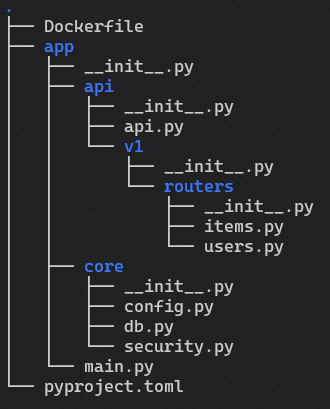
\includegraphics{images/backend-tree.png}
\paragraph{Dockerfile}
návod pro vytvoření Docker obrazu
\paragraph{app}
Python balíček
\paragraph{app/\_\_init\_\_.py}
dělá z "app" Python balíček
\paragraph{app/api}
Python subbalíček
\paragraph{app/api/\_\_init\_\_.py}
dělá z "app/api" Python subbalíček
\paragraph{app/api.py}
sdružuje všechny routery
\paragraph{app/main.py}
hlavní module, který vytváří "app" objekt
\subsubsection{Endpointy}
Všechny níže zmíněné endpointy obsahuje prefix https://www.domain.cz/api/v1
\paragraph{GET /items}
vrátí všechny položky
\paragraph{GET /items/:id}
vrátí položku s danným id
\paragraph{POST /items \{"param1": value, "param2": value\}}
vytvoří novou položku a vrátí ji
\paragraph{PUT /items/:id \{"param1": value, "param2": value\}}
upraví položku a vrátí ji
\paragraph{DELETE /items/:id}
odstraní položku a vrátí ji
\subsection{Kontejnerizace}
\paragraph{Kontejnerizace}
je technologie, která umožňuje izolovat aplikace do samostatných standardizovaných kontejnerů, což zjednodušuje jejich nasazení, škálování a správu. Každý kontejner obsahuje vše potřebné k běhu aplikace – kód, knihovny, systémové nástroje – a sdílí jádro operačního systému hostitele. Tato modularita umožňuje vývojářům snadno přenášet aplikace mezi různými vývojovými a produkčními prostředími, aniž by docházelo k problémům s kompatibilitou. Kontejnery jsou lehčí a flexibilnější než tradiční virtuální stroje, protože nevyžadují zbytečně těžký hypervizor. Mezi populární nástroje pro kontejnerizaci patří Docker a Kubernetes, které pomáhají automatizovat nasazování, škálování a správu kontejnerizovaných aplikací. Kontejnerizace tedy hraje klíčovou roli ve zjednodušení vývoje softwaru a zvyšování jeho efektivity.
\paragraph{Kontejner}
je standardizovaný ...
\subsubsection{Docker}
Docker představuje open source platformu sloužící k vývoji, distribuci a nasazení aplikací. Jeho klíčovou schopností je vytváření reprodukovatelných prostředí pro aplikace a jejich izolace od hostitelského systému. Tímto způsobem lze jednoduše "zabalit" aplikaci a nasadit ji na libovolném místě, kde je Docker dostupný. Díky izolaci a zabezpečení poskytované Dockerem lze na jednom hostiteli provozovat více instancí aplikací s minimálním rizikem interferencí mezi nimi. Docker funguje na principu takzvaných kontejnerů.
\paragraph{Dockerfile}
\paragraph{Docker image}
\paragraph{Docker Compose}
\subsection{Použité nástroje}
\paragraph{Git}
je open source, distribuovaný verzovní systém navržený i pro ty největší projekty.
\paragraph{GitHub}
jak už název napovída, je platforma pro správu softwarových projektů používající Git.  ... je největší kolaborativní platforma na správu převážně softwarových projektů, která je vlastněná firmou Microsoft. GitHub používá distribuovaný verzovací systém Git. GitHub nabízí... CI/CD pipelines - actions (linting, formatting, testing)
\paragraph{GitHub actions}je platforma pro continuous integration a continuous delivery (CI/CD), která umožňuje automatizovat build, testování a nasazení. Actions umožňují spouštět "workflows", když v repozitáři dojde k události např.: push, pull request. GitHub poskytuje Linux, MacOS nebo Windows virtuální zařízení pro spouštění těchto automatizací.
\paragraph{Visual Studio Code}
\paragraph{Docker Desktop}
\paragraph{Ruff}
\paragraph{pytest}
\paragraph{uv}
\paragraph{docker-compose}
\section{Zkratky}
open source
backend
frontend
framework
tech stack
\clearpage
\clearpage
\printbibliography
\end{document}
